% This work is licensed under the Creative Commons
% Attribution-NonCommercial-ShareAlike 4.0 International License. To view a copy
% of this license, visit http://creativecommons.org/licenses/by-nc-sa/4.0/ or
% send a letter to Creative Commons, PO Box 1866, Mountain View, CA 94042, USA.

\section{Aufgabenblatt 11}
\subsection*{Aufgabe $\ast$)}
Wir zeigen mit Hilfe des Pumpinglemmas, dass die Sprache $L:=\big\lbrace a^i ba^ib\mid i\in\N\big\rbrace$ nicht erkennbar ist.

\begin{proof}
	Widerspruchsbeweis: Angenommen $L$ ist erkennbar. Dann gilt nach Pumping\-lemma:
	Jedes Wort $\in L$ mit einer gewissen Länge lässt sich zerlegen in $w=xyz$ so, dass $xy^k z\in L$ liegt.
	Die einzig mögliche Zerlegung hierbei ist $y=a^iba^i$, da dies der einzige pumpbare Teil ist (nur $y=a^i$ geht auch nicht, da $x,z$ beim pumpen nicht "aufgeblasen" werden sollen).
	Somit ist $x=\varepsilon$ und $z=b$.
	Allerdings ist $a^iba^ia^ib a^ib=xy^2z\not\in L$.
	Widerspruch! Somit folgt die Behauptung.
\end{proof}

\subsection*{Aufgabe $\ast\ast$)}
Siehe Satz 4.1: 
Erkennbarkeit ist abgeschlossen unter $\cdot,\cap,\cup,\setminus,\overline{\cdot},\ast,\id$ (für Nerds: auch die symmetrische Differenz von zwei Sprachen ist wieder erkennbar. Man kann auch weitere eigene Operatoren definieren, z.B. Projektionen, etc.)\\
Konstruktionen der NEAs (in Worten):
\begin{itemize}
	\item $\cup$: neuer Startzustand, der mit $\varepsilon$-Transitionen zu beiden alten Startzuständen geht.
	\item $\overline{L}$ (Komplement): Mache DEA aus NEA (mit Potenzmengenkonstruktion).
	Dann ist der DEA für $\overline{L}$: $\overline{\A}:=\big(Q,\Sigma,q_0,\delta,Q\setminus F\big)$ ("flippe Endzustände")
	\item $\cap$: Produktautomat: $\A:=\big(Q_1\times Q_2,\Sigma,(q_{01},q_{02}),\Delta,F_1\times F_2\big)$
	\item $\setminus$: Folgt aus obigem, da $L_1\setminus L_2=L_1\cap\overline{L_2}$.
	\item $\cdot$ (Konkatenation): Die Endzustände des linken Automaten via $\varepsilon$-Transitionen mit Startzustand des rechten Automaten verbinden.
	\item $\ast$: Ergänze Start-End-Zustand $q_0$, der via $\varepsilon$-Transitionen mit Start- und Endzuständen des NEAs verbunden wird.
\end{itemize}

\subsection{Aufgabe 1}
Seien $r,s$ reguläre Ausdrücke, Beachte $r=s:\Longleftrightarrow L(r)=L(s)$ (eigentlich $r\equiv s$). Dann gilt:
\begin{enumerate}[label=\alph*)]
	\item $r+s=s+r$
	\item $(r+s)+t=r+(s+t)$
	\item $(rs)t=r(st)$
	\item $r(s+t)=rs+rt$
	\item $\emptyset^\ast=\varepsilon$
	\item $(r^\ast)^\ast=r^\ast$
	\item $r^\ast=rr^\ast+\varepsilon$
	\item $(\varepsilon+r)^\ast=r^\ast$
\end{enumerate}

\begin{proof}
	\underline{Zeige a):}
	\begin{align*}
		r+s
		\overset{\text{Not}}&=		
		L(r+s)
		\overset{\text{Def}}=
		L(r)\cup L(s)
		\overset{\text{Kommu. von }\cup}=
		L(s)\cup L(r)
		\overset{\text{Def}}=
		L(s+r)
		\overset{\text{Not}}=	
		s+r
	\end{align*}
	\underline{Zeige b):}
	\begin{align*}
		L\big((r+s)+t\big)
		\overset{\text{}}&=
		L(r+s)\cup L(t)\\
		\overset{\text{}}&=
		\big(L(r)\cup L(s)\big)\cup L(t)\\
		\overset{\text{Asso. von }\cup}&=
		L(r)\cup\big(L(s)\cup L(t)\big)\\
		\overset{\text{}}&=
		L(r)\cup L(s+t)\\
		\overset{\text{}}&=
		L\big(r+(s+t)\big)
	\end{align*}
	
	\underline{Zeige c):} "Ersetze Punkt durch Konkatenationsoperator auf Sprachen":
	\begin{align*}
		L\big((r\cdot s)\cdot t\big)
		\overset{\text{}}&=
		L(r\cdot s)\cdot L(t)\\
		\overset{\text{}}&=
		\big(L(r)\cdot L(s)\big)\cdot L(t)\\
		\overset{\text{}}&=
		\big\lbrace ab:a\in L(r)\cdot L(s)\wedge b\in L(t)\big\rbrace\\
		\overset{\text{}}&=
		\Big\lbrace ab:a\in\big\lbrace cd:c\in L(r)\wedge d\in L(s)\big\rbrace\wedge b\in L(t)\Big\rbrace\\
		\overset{\text{}}&=
		\Big\lbrace cdb:\big(c\in L(r)\wedge d\in L(s)\big)\wedge b\in L(t)\Big\rbrace\\
		\overset{\text{Asso. von }\wedge}&=
		\Big\lbrace cdb:c\in L(r)\wedge\big(d\in L(s)\wedge b\in L(t)\big)\Big\rbrace\\
		\overset{\text{}}&=
		\Big\lbrace ce:c\in L(r)\wedge e\in\big\lbrace db:d\in L(s)\wedge b\in L(t)\big\rbrace\Big\rbrace\\
		\overset{\text{}}&=
		\big\lbrace ce:c\in L(r)\wedge e\in L(s)\cdot L(t)\big\rbrace\\
		\overset{\text{}}&=
		L(r)\cdot\big(L(s)\cdot L(t)\big)\\
		\overset{\text{}}&=
		L(r)\cdot L(s\cdot t)\\
		\overset{\text{}}&=
		L\big(r\cdot(s\cdot t)\big)
	\end{align*}
	
	\underline{Zeige d):}
	\begin{align*}
		L\big(r(s+r)\big)
		\overset{\text{Def}}&=
		L(r)\cdot L(s+t)\\
		\overset{\text{}}&=
		L(r)\cdot\big(L(s)\cup L(t)\big)\\
		\overset{\text{Aufgabe 7.2 (a)}}&=
		L(r)\cdot L(s)\cup L(r)\cdot L(t)\\
		\overset{\text{}}&=
		L(r\cdot s)\cup L(r\cdot t)\\
		\overset{\text{}}&=
		L(rs+rt)
	\end{align*}		
	
	\underline{Zeige e):}
	Achtung! Hier ist \underline{nicht} der Kleene-Stern gemeint. 
	Er ist definiert als der Kleene-Stern der Sprache,
	\begin{align*}
		L(\underbrace{\emptyset^\ast}_{\text{Regex}})
		\overset{\text{\Def}}&=
		L(\underbrace{\emptyset}_{\text{Regex}})^\ast
		\overset{\text{\Def}}=
		\underbrace{\emptyset^\ast}_{\text{Sprache}}
		\overset{\text{Def }\ast}=
		\bigcup\limits_{n=0}^\infty
		\overset{\text{}}=
		\varepsilon\cup\emptyset\cup\ldots
		\overset{\text{}}=
		\lbrace\underbrace{\varepsilon}_{\text{leeres W}}\rbrace
		\overset{\text{\Def}}=
		L(\underbrace{\varepsilon}_{\text{Regex}})
	\end{align*}
	
	\underline{Zeige f):}
	\begin{align*}
		L\big((r^\ast)^\ast\big)
		\overset{\text{}}&=
		L(r^\ast)^\ast
		\overset{\text{}}=
		\big(L(r)^\ast\big)^\ast
		\overset{\text{Aufg 7.2 (d)}}=
		L(r)^\ast
		\overset{\text{}}=
		L(r^\ast)
	\end{align*}
	Beachte: Alle $\ast$-Symbole innerhalb $L(\ldots)$ bezeichnen den Sternoperator der regulären Ausdrücke.
	Alle $\ast$-Symbole außerhalb $L(\ldots)$ bezeichnet den Kleene-Stern.
	
	\underline{Zeige g):}
	\begin{align*}
		L(r^\ast)
		\overset{\text{}}&=
		L(r)^\ast\\
		\overset{\text{}}&=
		\bigcup\limits_{n=0}^\infty L(r)^n\\
		\overset{\text{}}&=
		L(r)^0\cup\bigcup\limits_{n=1}^\infty L(r)^n\\
		\overset{\text{}}&=
		L(r)^0\cup L(r)\cdot\left(\bigcup\limits_{n=0}^\infty L(r)^n\right)\\
		\overset{\text{}}&=
		\lbrace\varepsilon\rbrace\cup L(r)\cdot L(r)^\ast\\
		\overset{\text{}}&=
		L(\varepsilon)\cup L(r)\cdot L(r^\ast)\\
		\overset{\text{}}&=
		L(\varepsilon)\cup L(r\cdot r^\ast)\\
		\overset{\text{}}&=
		L(\varepsilon+rr^\ast)\\
		\overset{\text{a)}}&=
		L(rr^\ast+\varepsilon)
	\end{align*}
	
	\underline{Zeige h):}
	\begin{align*}
		L\big((\varepsilon+r)^\ast\big)
		\overset{\text{}}&=
		L(\varepsilon+r)^\ast\\
		\overset{\text{}}&=
		\big(L(\varepsilon)\cup L(r)\big)^\ast\\
		\overset{\text{}}&=
		\big(\lbrace\varepsilon\rbrace\cup L(r)\big)^\ast\\
		\overset{\text{}}&=
		L(r)^\ast\\
		\overset{\text{}}&=
		L(r^\ast)
	\end{align*}
\end{proof}

\subsection{Aufgabe 2}
Verwenden Sie die Konstruktion aus dem Beweis von Satz von Kleene (Satz 5.4) und das
Lemma von Arden (Lemma 5.6), um einen regulären Ausdruck $r$ anzugeben, der die von dem
folgenden Automaten $\A$ akzeptierte Sprache repräsentiert (das heißt, es soll $L(r) = L(\A)$ gelten).

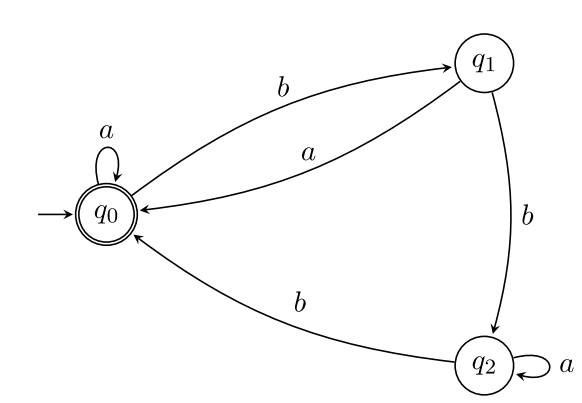
\includegraphics[width=0.7\textwidth]{pics/Blatt11_2.png}
 
\begin{lösung}
	\textbf{Lemma von Arden:}
	Seien $A,B\subseteq\Sigma^\ast$ und $\varepsilon\not\in A$.
	Dann hat
	\begin{align}\label{eqLemmaArden}\tag{Arden}
		X=A\cdot X\cup B
	\end{align}
	die eindeutige Lösung $X=A^\ast\cdot B$.\nl
	Wir erzeugen nun für jeden Zustand $q\in Q$ eine Gleichung.
	\begin{align}\label{eq2_1}
		X_0&=\lbrace a\rbrace\cdot X_0\cup\lbrace b\rbrace\cdot X_1\cup\lbrace\varepsilon\rbrace\\\label{eq2_2}
		X_1&=\lbrace a\rbrace\cdot X_0\cup\lbrace b\rbrace\cdot X_2\\
		X_2&=\lbrace a\rbrace\cdot X_2\cup\lbrace b\rbrace\cdot X_0\label{eq2_3}
	\end{align}
	Notizen:
	\begin{itemize}
		\item Bei Endzuständen muss $\cup\lbrace\varepsilon\rbrace$ ergänzt werden.
		\item Man schaut sich alle ausgehenden Transitionen an.
	\end{itemize}
	Wende nun Lemma von Arden auf \eqref{eq2_3} an:
	\begin{align}\label{eq2_4}
		X_2&=\lbrace a\rbrace^\ast\cdot\lbrace b\rbrace\cdot X_0 &\text{Lemma auf \eqref{eq2_3}}\\%\nonumber
		X_1&=\lbrace a\rbrace\cdot X_0\cup\lbrace b\rbrace\cdot\lbrace a\rbrace^\ast\cdot\lbrace b\rbrace\cdot X_0 &\text{Einsetzen von \eqref{eq2_4} in \eqref{eq2_2}}\\
		&=\Big(\lbrace a\rbrace\cup\lbrace b\rbrace\cdot\lbrace a\rbrace^\ast\cdot\lbrace b\rbrace\Big)\cdot X_0\label{eq2_5}\\
		X_0&=\lbrace a\rbrace\cdot X_0\cup\lbrace b\rbrace\Big(\lbrace a\rbrace\cup\lbrace b\rbrace\cdot\lbrace a\rbrace^\ast\cdot\lbrace b\rbrace\Big)\cdot X_0\cup\lbrace\varepsilon\rbrace &\text{Einsetzen von \eqref{eq2_5} in \eqref{eq2_1}}\nonumber\\
		\overset{\text{Distr}}&{=}
		\Big(\lbrace a\rbrace\cup\lbrace b\rbrace\cdot\big(\lbrace a\rbrace\cup\lbrace b\rbrace\cdot\lbrace a\rbrace^\ast\cdot\lbrace b\rbrace\big)\Big)\cdot X_0\cup\lbrace\varepsilon\rbrace\label{eq2_6}\\
		X_0&=\Big(\lbrace a\rbrace\cup\lbrace b\rbrace\cdot\big(\lbrace a\rbrace\cup\lbrace b\rbrace\cdot\lbrace a\rbrace^\ast\cdot\lbrace b\rbrace\big)\Big)^\ast\cdot\lbrace\varepsilon\rbrace &\text{Lemma auf \eqref{eq2_6}}\nonumber\\
		&=L\Big(\big(a+b\cdot(a+ba^\ast b)\big)^\ast\Big)\nonumber\\
		&=L\Big(\big(a+ba+bba^\ast b\big)^\ast\Big)\nonumber
	\end{align}
\end{lösung} 

\subsection{Aufgabe 3}
Sei $\Sigma=\lbrace a,b,c\rbrace$.
 Geben Sie für jede der folgenden Sprachen $L_i$ einen regulären Ausdruck $r_i$ mit $L_i=L(r)$ an.
Erklären Sie die Wahl Ihrer regulären Ausdrücke $r_i$.

\begin{enumerate}[label=\alph*)]
	\item $L_1=\big\lbrace w\in\Sigma^\ast:w\text{ beginnt mit $a$ mit $|w|_b$ ist gerade}\big\rbrace$
	\item $L_2=\big\lbrace w\in\Sigma^\ast:\nexists u,v\in\Sigma^\ast:w=uaav\big\rbrace$
\end{enumerate}

\begin{lösung}
	Idee: 
	\begin{enumerate}
		\item Konstruiere NEA $\A_i$ mit $L(\A_i)=L_i$.
		\item Ermittle den regulären Ausdruck $r_i$ von $\A_i$ wie in Aufgabe 2.
	\end{enumerate}		

	\underline{Zeige a):}
	
	\usetikzlibrary{positioning,automata}
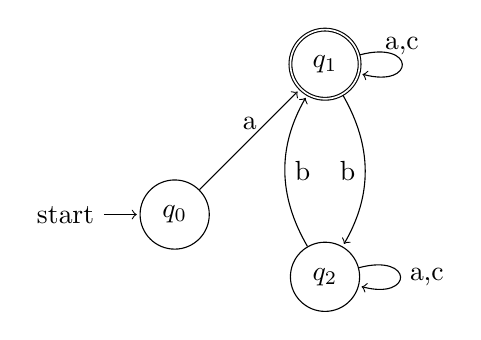
\begin{tikzpicture}[shorten >=1pt,node distance=2.7cm,on grid]
  \node[state,initial]   	(q_0)                		{$q_0$};
  \node[state, accepting] 	(q_1) [above right=of q_0] 	{$q_1$};
  \node[state] 	(q_2) [below=of q_1] 		{$q_2$};
  \path[->] (q_0) edge [bend left=0] node [above] {a} (q_1)
            (q_1) edge [loop right] node [above] {a,c} ()
            	  edge [bend left=30] node [left] {b} (q_2)
            (q_2) edge [loop right] node [right] {a,c} ()
                  edge [bend left=30] node [right] {b} (q_1)
       ;
\end{tikzpicture}

	$q_1\hat{=}$ "gerade Anzahl von b's gelesen"\\
	$q_2\hat{=}$ "ungerade Anzahl von b's gelesen"
	
	\begin{align}
		X_0&=\lbrace a\rbrace\cdot X_1\\
		X_1&=\lbrace a,c\rbrace\cdot X_1\cup\lbrace b\rbrace\cdot X_2\cup\lbrace\varepsilon\rbrace\\
		X_2&=\lbrace a,c\rbrace\cdot X_2\cup\lbrace b\rbrace\cdot X_1
	\end{align}
	
	Mit dem Lemma von Arden erhalten wir (anwenden auf letzte Gleichung):
	\begin{align*}
		X_2&=\lbrace a,c\rbrace^\ast\cdot\lbrace b\rbrace\cdot X_1\\
		X_1&=\lbrace a,c\rbrace\cdot X_1\cup\lbrace b\rbrace\cdot\lbrace a,c\rbrace^\ast\cdot\lbrace b\rbrace\cdot X_1\cup\lbrace\varepsilon\rbrace\\
		&=\Big(\lbrace a,c\rbrace\cup\lbrace b\rbrace\cdot\lbrace a,c\rbrace^\ast\cdot\lbrace b\rbrace\Big)\cdot X_1 \cup\lbrace\varepsilon\rbrace\\
		X_1&=\Big(\lbrace a,c\rbrace\cup\lbrace b\rbrace\cdot\lbrace a,c\rbrace^\ast\cdot\lbrace b\rbrace\Big)^\ast\cdot\lbrace\varepsilon\rbrace\\
		X_0&=\lbrace a\rbrace\cdot\Big(\lbrace a,c\rbrace\cup\lbrace b\rbrace\cdot\lbrace a,c\rbrace^\ast\cdot\lbrace b\rbrace\Big)^\ast\\
		&=L\Big(a\cdot\big((a+c)+b(a+c)^\ast b\big)^\ast\Big)=:r_i
	\end{align*}		
	
	\underline{Zeige b):}
	Sprache umschreiben:
	\begin{align*}
		L_2&=\big\lbrace w\in\Sigma^\ast:\nexists u,v\in\Sigma^\ast:w=uaav\big\rbrace\\
		&=\big\lbrace w\in\Sigma^\ast: w\text{ enthält keine zwei aufeinanderfolgenden $a$'s}\big\rbrace
	\end{align*}
	
	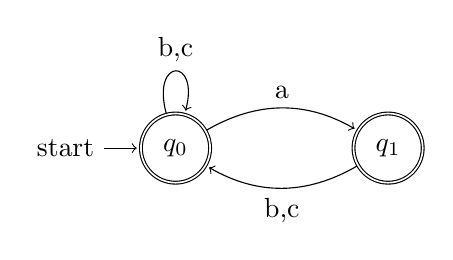
\begin{tikzpicture}[shorten >=1pt,node distance=2.7cm,on grid]
  \node[state,initial, accepting](q_0)           		{$q_0$};
  \node[state, accepting] 	(q_1) [right=of q_0] 	{$q_1$};
  \path[->] (q_0) edge [loop above] node [above] {b,c} ()
  				  edge [bend left=30] node [above] {a} (q_1)
            (q_1) edge [bend left=30] node [below] {b,c} (q_0)
       ;
	\end{tikzpicture}

	\begin{align*}
		r_1=\big(b+c+a\cdot(b+c)\big)^\ast\cdot(a+\varepsilon)
	\end{align*}
	
	
\end{lösung}

